%!TeX root = Chapter_Data2
\documentclass[../../CompleteThesis2/Complete_2ndDraft]{subfiles}
%\graphicspath{{../../Figures/}}
\begin{document}

\section[Volcanic Horizons][Volcanic Horizons]{Determining Time of Volcanic Material Deposition}
\label{Sec:Data_VolcanicHorizons}

\begin{figure}[h]
	\centering
	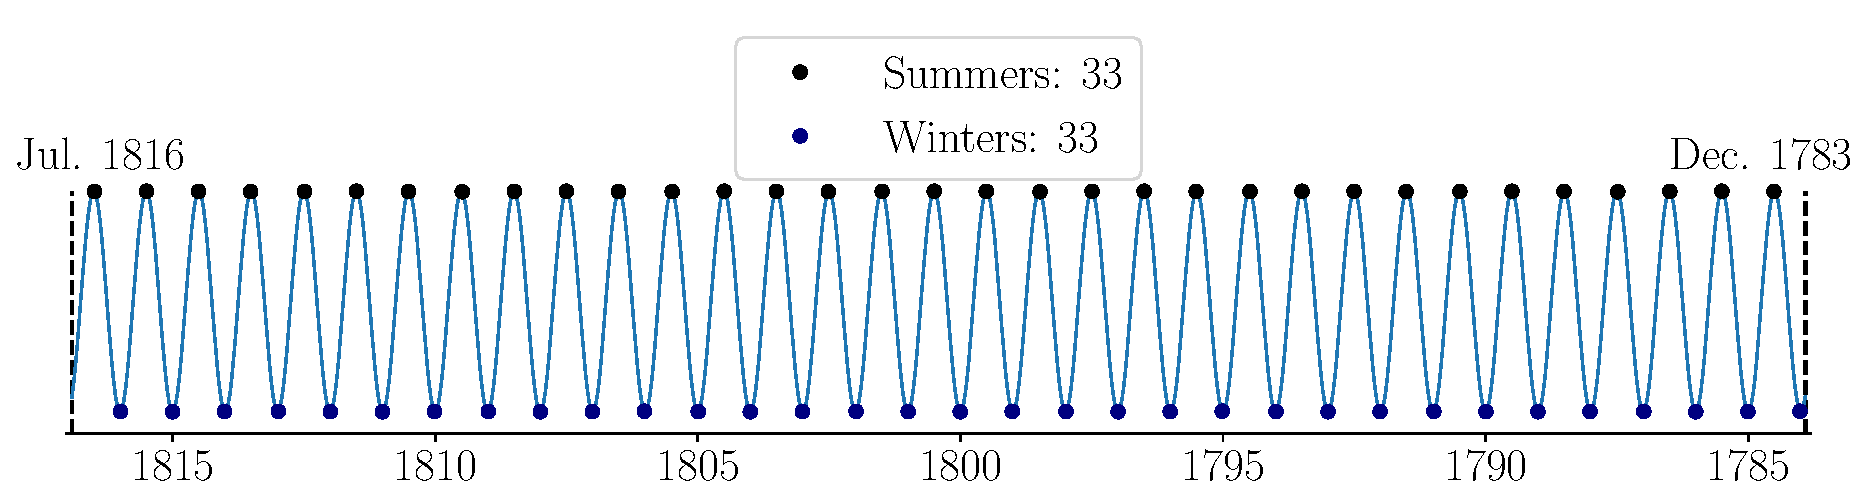
\includegraphics[width=\textwidth]{summersWinters_LT.pdf}
	\caption[Summers and Winters between Laki and Tambora]{\small Illustration of expected summers and winters in the time span between the Laki and Tambora volcanic depositions in Greenland.}
	\label{Fig:SummersAndWintersLT}
\end{figure}

For this thesis, two volcanic horizons have been in focus, namely the eruption of the Icelandic volcano Laki in 1783 and the Indonesian volcano Tambora in 1815. Due to delay in atmospheric transport (\cite[Wei et al., 2008]{Wei2008}, \cite[Cole-Dai et al, 2009]{Dai2009}), the volcanic material from Tambora was first deposited around the summertime of 1816. This reveals a time span between volcanic material deposition from the two eruptions of 33 summers(peaks) and 33 winters(troughs).The essence of this project is to restore as much of the diffused signal as possible, while obeying the constraint, that the isotopic signal must correspond to this time span, that is, the signal must exhibit 33 peaks and 33 troughs.


\begin{figure}[h]
	\centering
	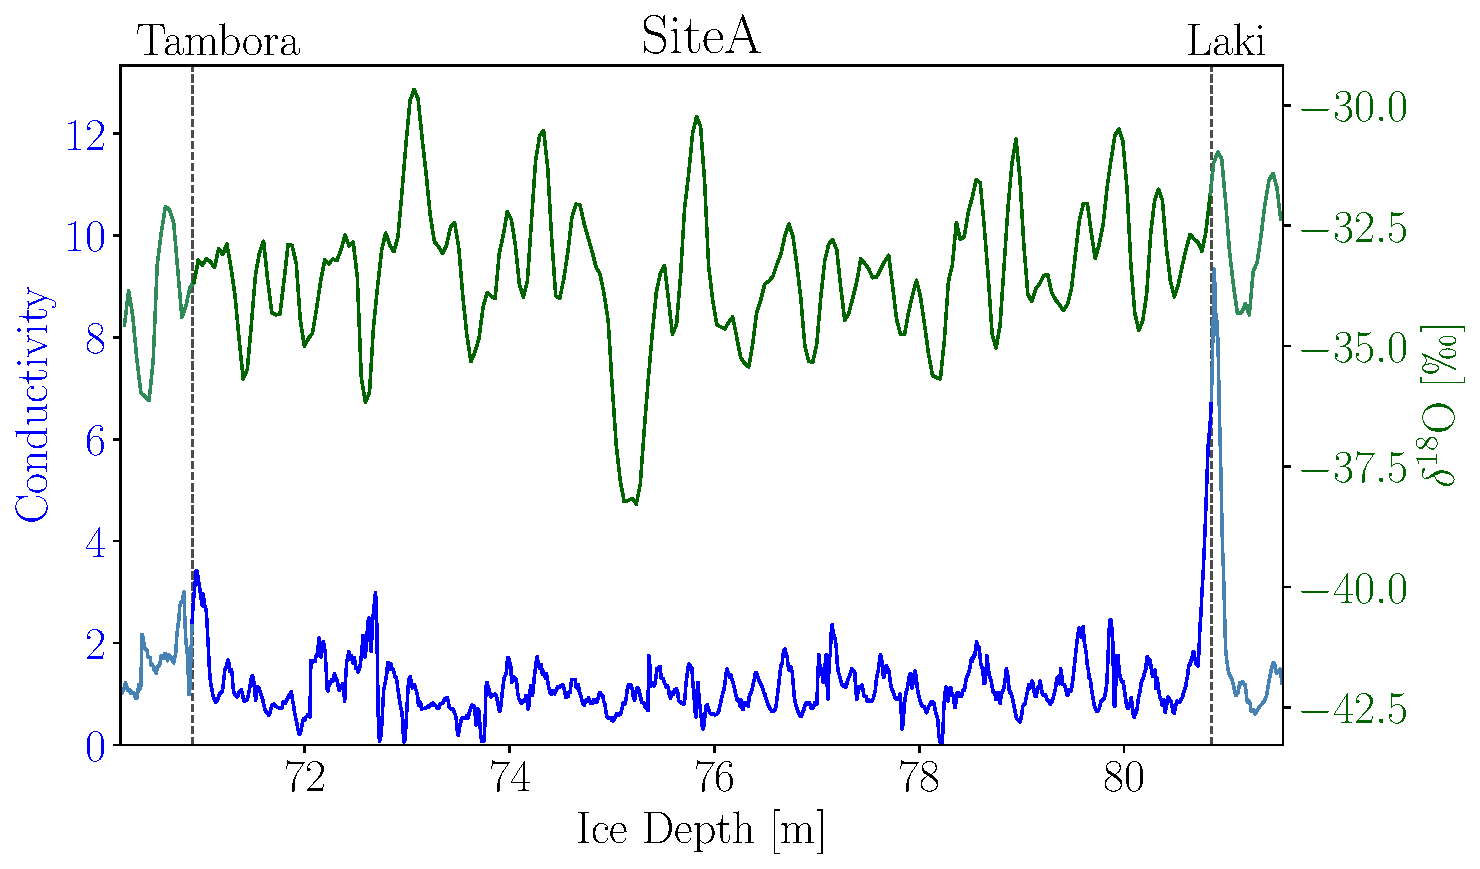
\includegraphics[width=0.9\textwidth]{SiteA_ECMd18O_combo.pdf}
	\caption[ECM and $\delta^{18}$O data between Laki and Tambora, Site A.]{\small Conductivity measurements aligned with water isotope measurements at the depth correspodning to the time between eruptions at Laki and Tambora.}
	\label{Fig:DATA_SiteA_ECM_d18O_combo}
\end{figure}
In Figure \ref{Fig:DATA_SiteA_ECM_d18O_combo}, the isotopic and the conductivity signals have been aligned from the assumed positions of the Laki and Tambora depositions. The Laki deposition signal is especially well-defined, as it originates from a volcano in the vicinity of the Greenlandic ice core. The Tambora signal on the other hand is more smudged and has a wider signal with a less well-defined peak. This is due to the large hemispheric distance between Greenland and Indonesia, and the time it thus takes for the volcanic material to be distributed through the atmosphere and finally deposited at Greenland.



Specifically considering the constraint involving the 33 troughs, there might be room for some error, as it is clear that if the deposition happened just a bit earlier or later than expected, there might one or two troughs more or less. 

\subsection[Corrected Depth]{Corrected Depth Estimate}
\label{Subsec:Data_VolcanicHorizons_CorrDepthEst}

\cite[Clausen \& Hammer, 1988]{ClausenHammer1988} presented estimates of the Laki and Tambora positions from the ECM measurements previously presented in this thesis. These positions have in this thesis been revisited and corrected to a more fitting central value, which can be seen in Figure \ref{fig:LakiTambDepths_corr} and Table \ref{Tab:LakiTamb_corr}. In the table the subscript 'CH' refers to values as found in \cite[Clausen \& Hammer, 1988]{ClausenHammer1988} and subscript 'TQ' refers to new estimates as found in this thesis. $m$ corresponds to what is estimated to be middle of the event and $s$ corresponds to the estimated width of the event.

\begin{figure}[h]
	\centering
	\begin{subfigure}{.45\textwidth}
		\centering
		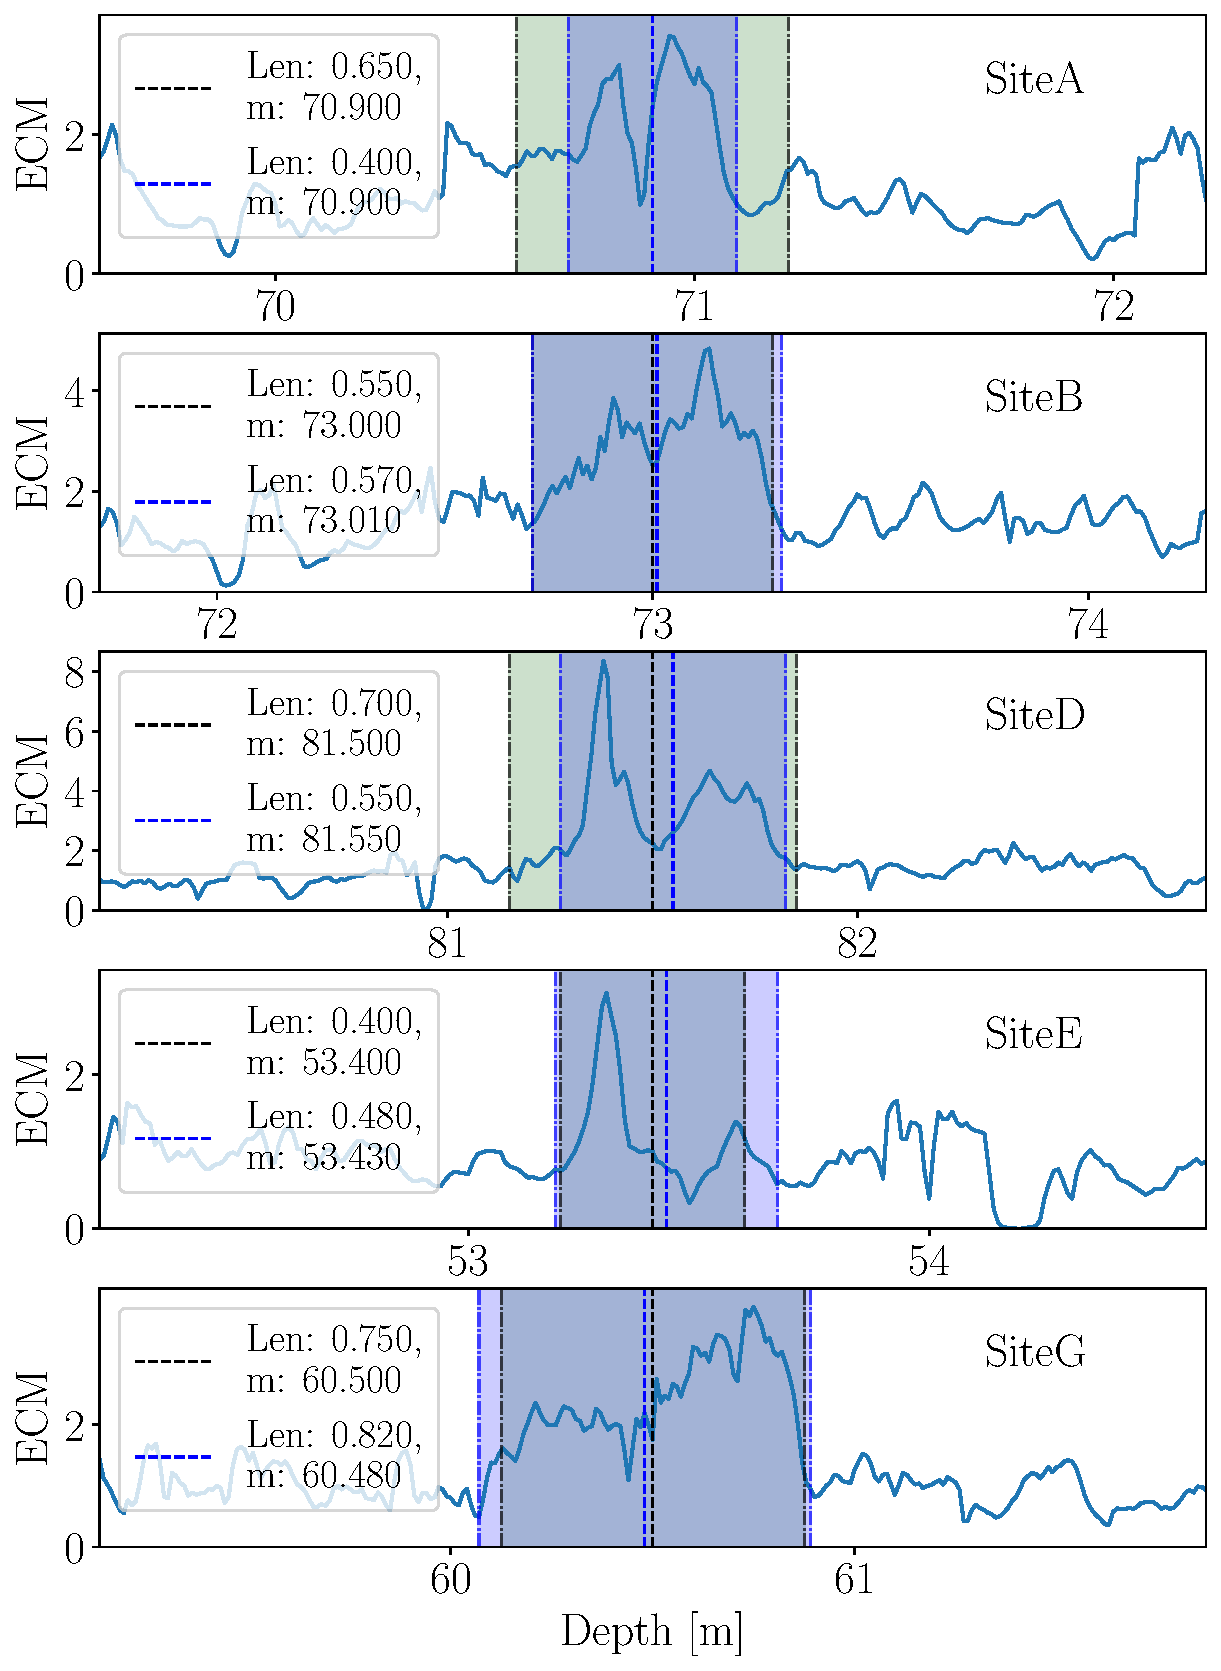
\includegraphics[width=\textwidth]{TambDepth_corr.pdf}
		\caption[Corrected Tambora locations.]{\footnotesize Corrected depth positions and duration for Tambora deposition event.}
		\label{fig:DATA_TambDepth_corr}
	\end{subfigure}
	~
	\begin{subfigure}{.45\textwidth}
		\centering
		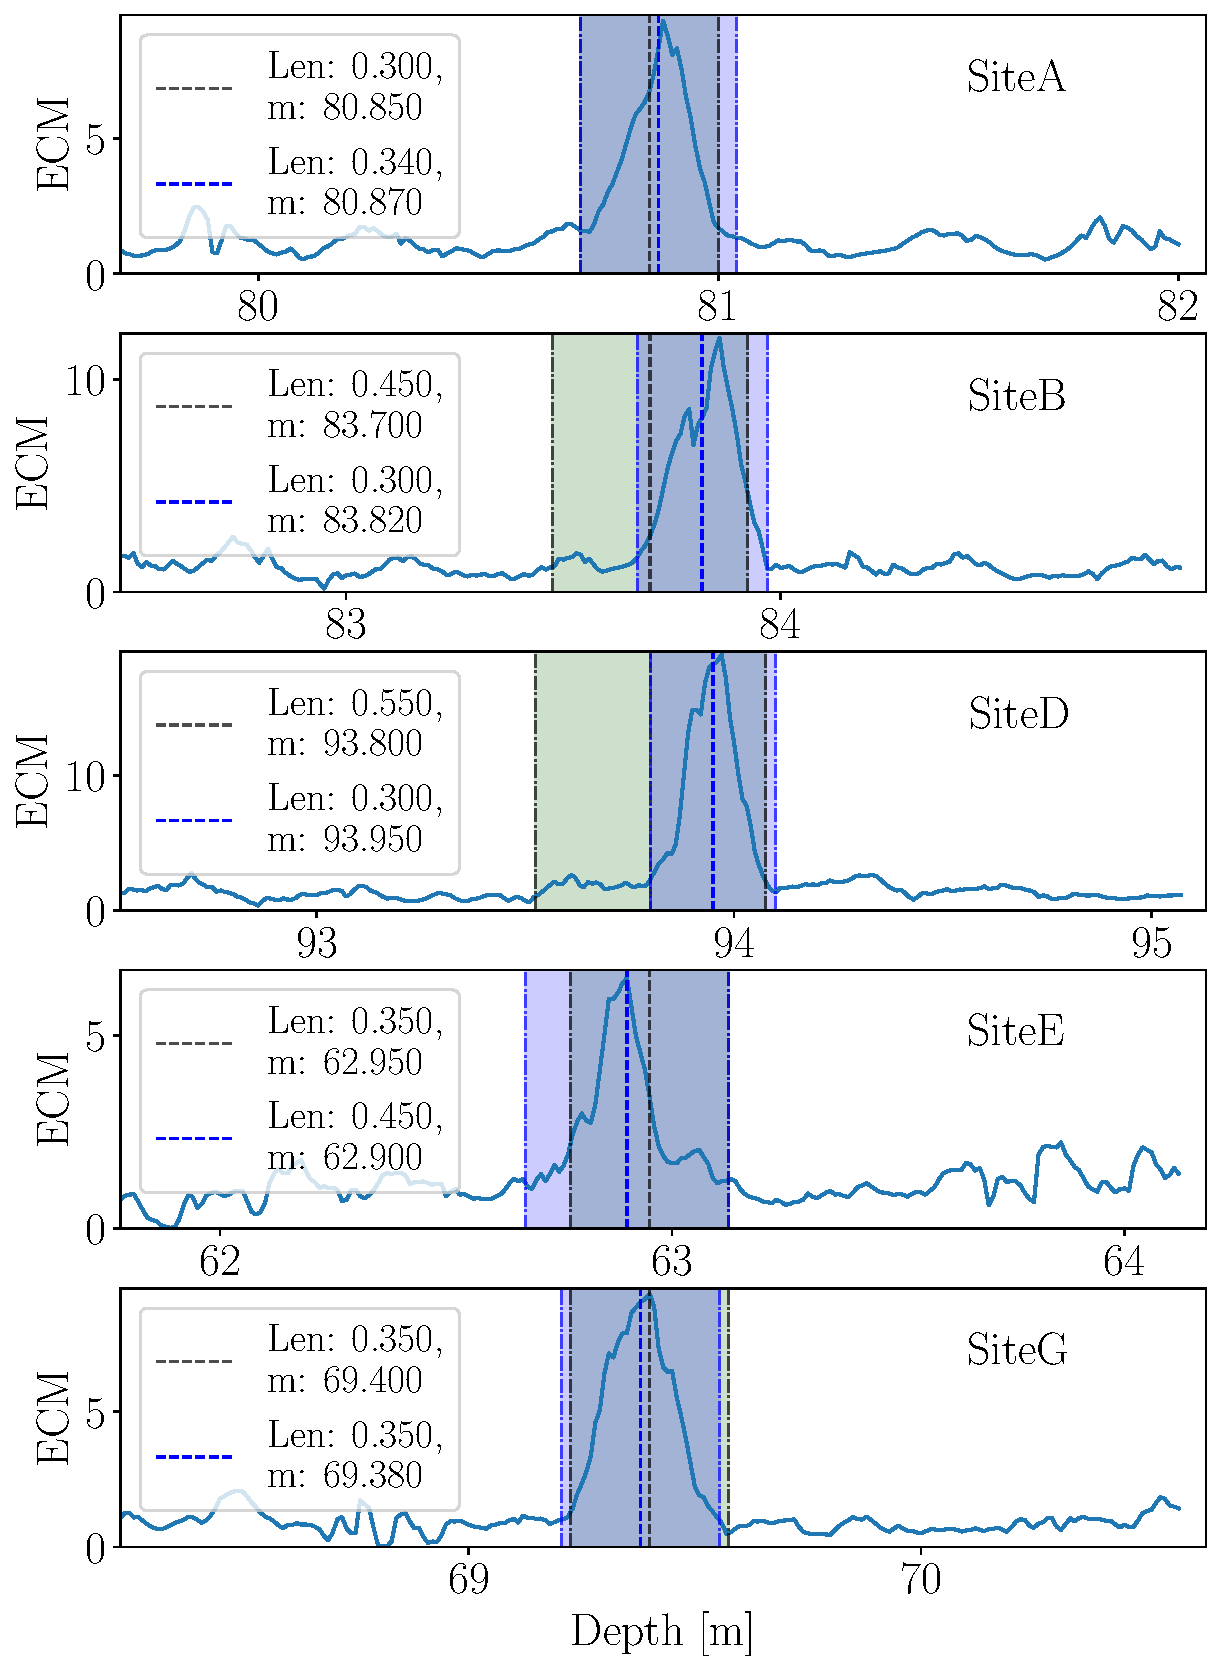
\includegraphics[width=\textwidth]{LakiDepth_corr.pdf}
		\caption[Corrected Laki locations.]{\footnotesize Corrected depth positions and duration for Laki deposition event.}
		\label{fig:DATA_LakiDepth_corr}
	\end{subfigure}
	\caption[Corrected depth positions of Laki and Tambora events.]{\small Corrected depth positions durations for the volcanic signal of Laki and Tambora in the ECM data. Green shades corresponds to previously estimated depths, from \cite[Clausen \& Hammer, 1988]{ClausenHammer1988}, and blue shades corresponds to newly estimated positions and durations.}
	\label{fig:DATA_LakiTambDepths_corr}
\end{figure}

\begin{table}[h]
	\centering
	\begin{tabular}{l|cc|cc|cc|cc|}
		& \multicolumn{4}{c|}{Tambora} & \multicolumn{4}{c|}{Laki}\\
		Core & $m_{\text{CH}}$ & $m_{\text{TQ}}$ & $s_{\text{CH}}$ & $s_{\text{TQ}}$& $m_{\text{CH}}$ & $m_{\text{TQ}}$ & $s_{\text{CH}}$ & $s_{\text{TQ}}$ \\
		 & [m] & [m] & [m] & [m]& [m] & [m] & [m] & [m] \\
		\hline
		Site A & 70.90 & 70.90 & 0.65 & 0.40 & 80.85 & 80.87 & 0.30 & 0.34 \\
		Site B & 73.00 & 73.01 & 0.55 & 0.57 & 83.70 & 83.82 & 0.45 & 0.30 \\	
		Site D & 81.50 & 81.55 & 0.55 & 0.70 & 93.80 & 93.95 & 0.55 & 0.30 \\
		Site E & 53.40 & 53.43 & 0.40 & 0.48 & 62.95 & 62.90 & 0.35 & 0.45 \\
		Site G & 60.50 & 60.48 & 0.75 & 0.82 & 69.40 & 69.38 & 0.35 & 0.35 \\
	\end{tabular}
	\caption[Corrected Laki and Tambora positions.]{\footnotesize Original and corrected middle, $m$, and width, $s$, values for Laki and Tambora deposition events.}
	\label{Tab:LakiTamb_corr}
\end{table}



\subsection[Gaussian Distribution]{Gaussian Distribution}
\label{Subsec:Data_VolcanicHorizons_GaussDist}


From the corrected middle and width estimates for the volcanic events observed in ECM data, it is possible to investigate what happens to the further analysis if the event location is moved from a fixed point. This gives a possibility of estimating the locations as Gaussian distributions, with a mean equal to the middle value and a standard deviation of $1/4$ (Tambora) or $1/5$ (Laki) of the width, and thus makes it possible to draw the laki and Tambora locations from these distributions. This enables further analysis of the developed method, as the stability can be tested by varying the positions of the volcanic events within these Gaussian distributions. To be able to use the developed method, it might be necessary to make the constraints of 33 peaks and 33 troughs soft but the stability of these constraints is also something that can be investigated through this method. Figures \ref{Fig:DATA_SiteA_LakiDepth_Gauss} and \ref{Fig:DATA_SiteA_TambDepth_Gauss} show examples of Gaussian distributions generated from investigation of midpoint and width of the volcanic events. 

\begin{marginfigure}
	\centering
	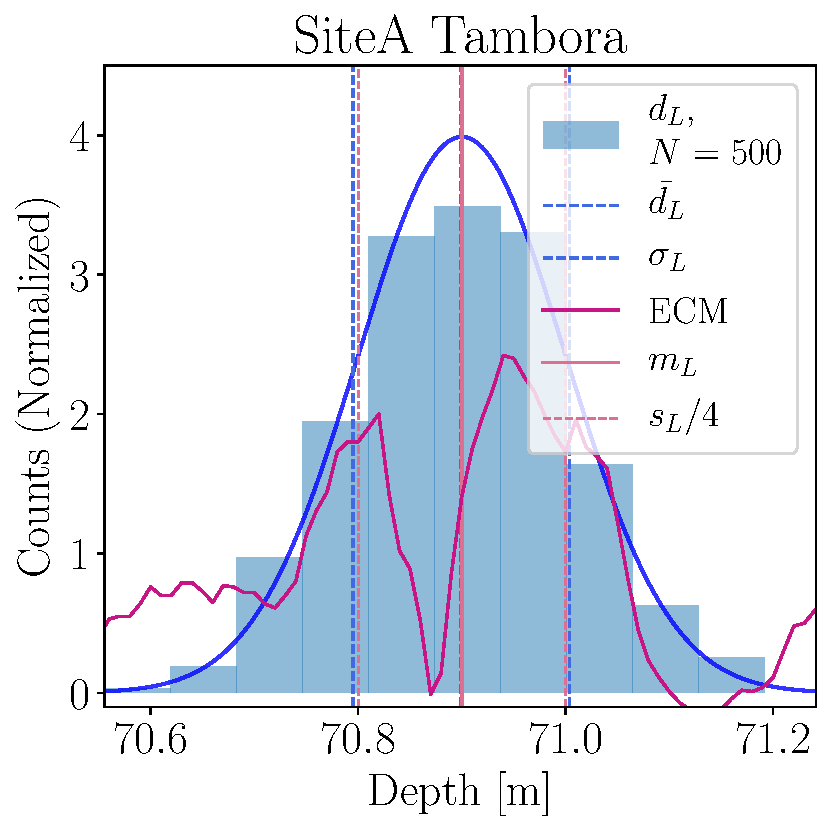
\includegraphics[width=\marginparwidth]{SiteATambDepth_Gauss.pdf}
	\caption[Corrected Tambora event, Site A.]{\footnotesize Example of Gaussian distribution of the volcanic event from Tambora,  enerated from observations of the ECM data, Site A. $\mu_T$ for the distribution is set to be equal to the middle point, $s_T$, and the standard deviation, $\sigma_T^2$ is set to be $s_T/4$.}
	\label{Fig:DATA_SiteA_TambDepth_Gauss}
\end{marginfigure}


\begin{marginfigure}
	\centering
	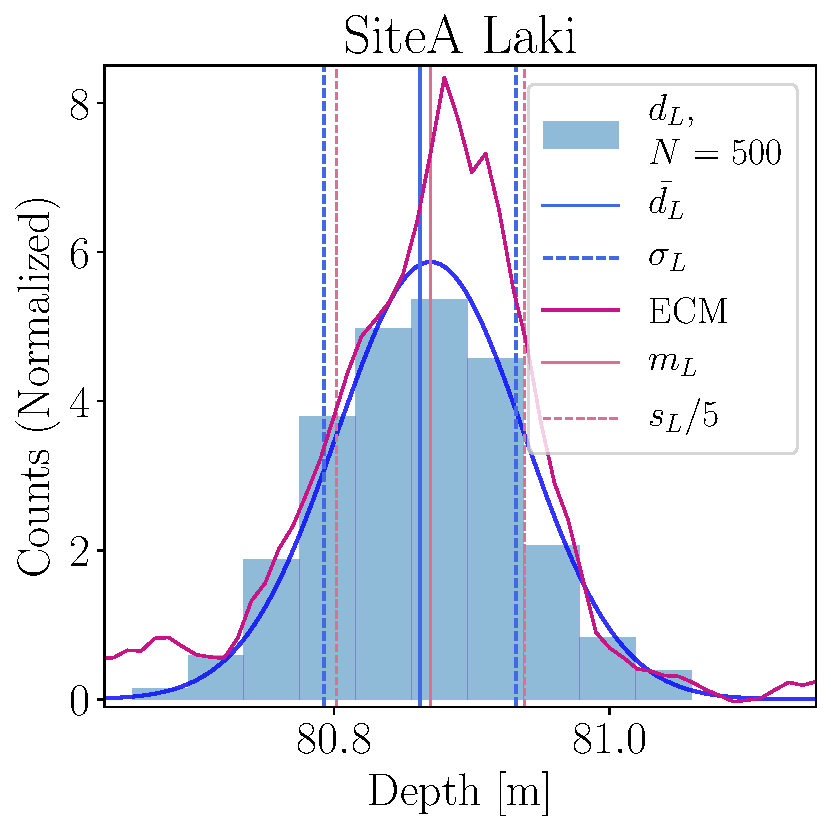
\includegraphics[width=\marginparwidth]{SiteALakiDepth_Gauss.pdf}
	\caption[Corrected Laki event, Site A.]{\footnotesize Example of Gaussian distribution of the volcanic event from Laki,  enerated from observations of the ECM data, Site A. $\mu_L$ for the distribution is set to be equal to the middle point, $s_L$, and the standard deviation, $\sigma_L^2$ is set to be $s_L/5$.}
	\label{Fig:DATA_SiteA_LakiDepth_Gauss}
\end{marginfigure}



\section[Selection][Selection]{Selection of Isotopic Data}
\label{Sec:Data_Selection}


The method developed in this project is very general and can hopefully be used for information reconstruction and diffusion length estimation in a great number of different ice cores. But to develop a general algorithm one must first test it on specific data sets. I chose to focus mainly on a number of shallow ice cores, the Alphabet cores near the Greenlandic ice core Crete, and especially on the core drilled at Site A, see Figure \ref{Alphabet_Map} for location of the different cores examined.

\subsection[AWI B-cores]{AWI B-cores: Core B23}
\label{Subsec:Data_Selection_Bcores}
%\todo{DATA: Make spatial map of B-cores locations.}


Before choosing to focus mainly on the Alphabet cores, some time was spend on examining a number of cores of length between 100-175 m drilled during the North Greenland Transverse (NGT) between 1993 and 1995 in northern Greenland, from now on referred to as the AWI (Alfred-Wegener-Institut) B-cores, \cite[Weissbach et al. 2016]{Weissbach2016}. These were primarily chosen due to their great spatial coverage of an area of roughly 10 \% of the Greenland ice sheet. This could have proven very useful for using the method developed here to estimate a spatial-temporal map of the covered area in the period between the eruptions of Laki and Tambora. Unfortunately the data from the AWI B-cores where not of high enough quality to meet the requirements of the following data analysis. Of the twelve AWI B cores available, only seven had corresponding electrical conductivity measurements with recognizable Laki and Tambora signals. Out of these seven only three were of adequate quality and resolution to subsequently be analyzed, see Appendix \ref{App:Data_AWI}. The $\delta^{18}$O and electrical conductivity profiles of one of the three high-quality cores from the NGT can be seen in Figure \ref{fig:B23_ECMd18O_combo}.

\begin{figure}[h]
	\centering
	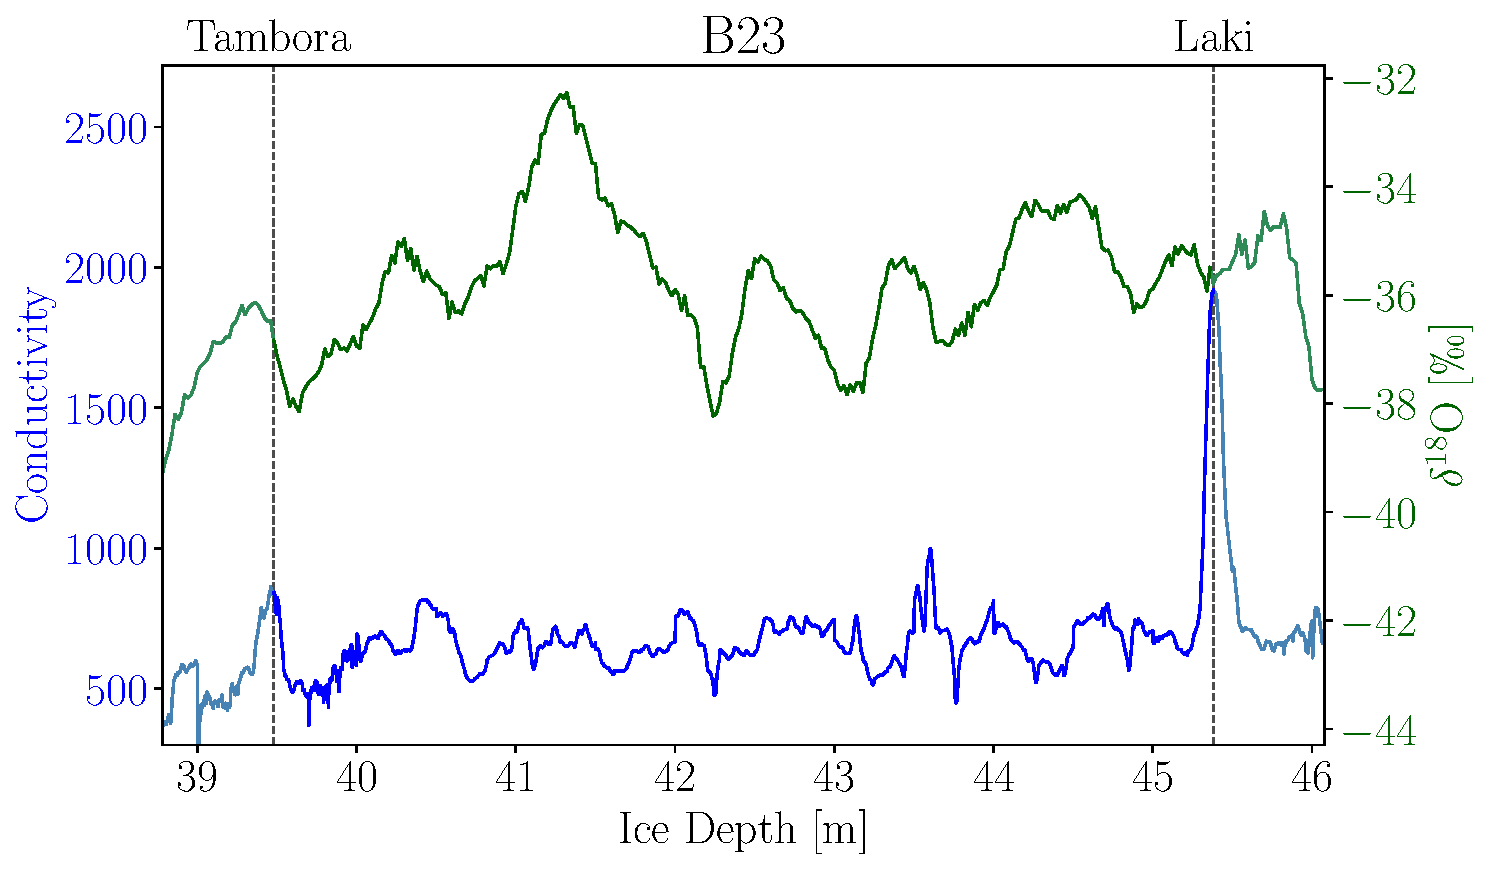
\includegraphics[width=0.8\textwidth]{B23_ECMd18O_combo.pdf}
	\caption[ECM and $\delta^{18}$O data between Laki and Tambora, Site B23.]{\small $\delta^{18}$O and conductivity profile of the AWI B-core B23. The dashed lines represent the suggested locations of the Laki and Tambora eruptions as matched in \cite[Weissbach et al. 2016]{Weissbach2016}}
	\label{fig:B23_ECMd18O_combo}
\end{figure}


\subsection[Crete Area][Crete Area]{Crete and Surrounding Alphabet Cores: Site A}
\label{Subsec:Data_Selection_Alhabet}
\begin{marginfigure}
	\centering
	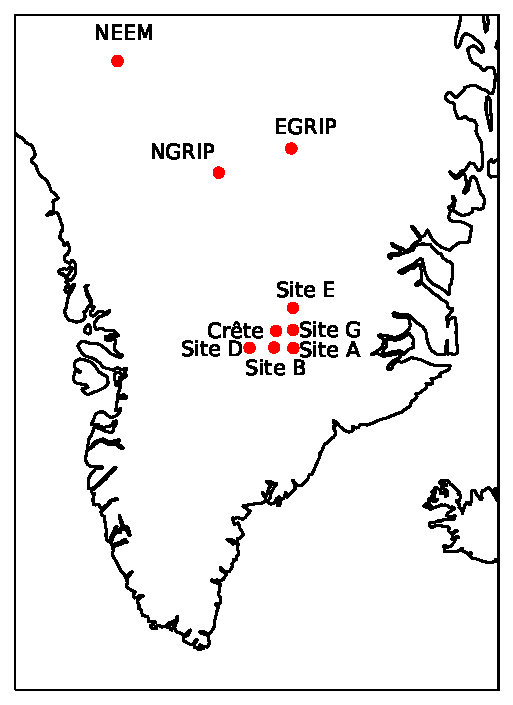
\includegraphics[width=\marginparwidth]{AlphabetCores1.pdf}
	\caption[]{\footnotesize Location of Alphabet cores along with some major ice cores, NEEM, EGRIP and NGRIP.}
	\label{Fig:AlphabetCoresMap}
\end{marginfigure}

\begin{figure}[!htb]
	\centering
	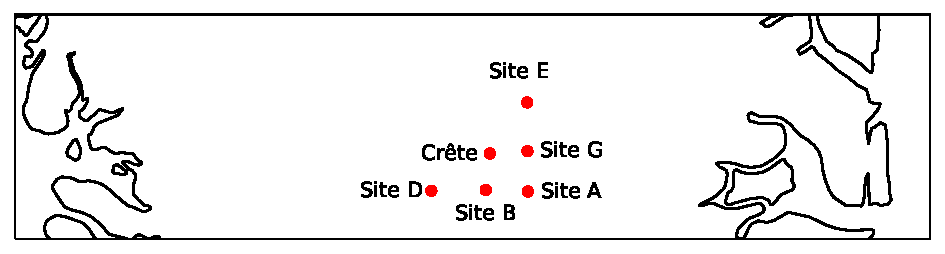
\includegraphics[width=0.95\textwidth]{AlphabetCores1_Zoom.pdf}
	\caption[Alphabet Cores Map]{\small Map of spatial locations of the Alphabet cores analyzed in this thesis.}
	\label{Fig:MapAlphabetCores}
\end{figure}


\begin{figure}[!htb]
	\centering
	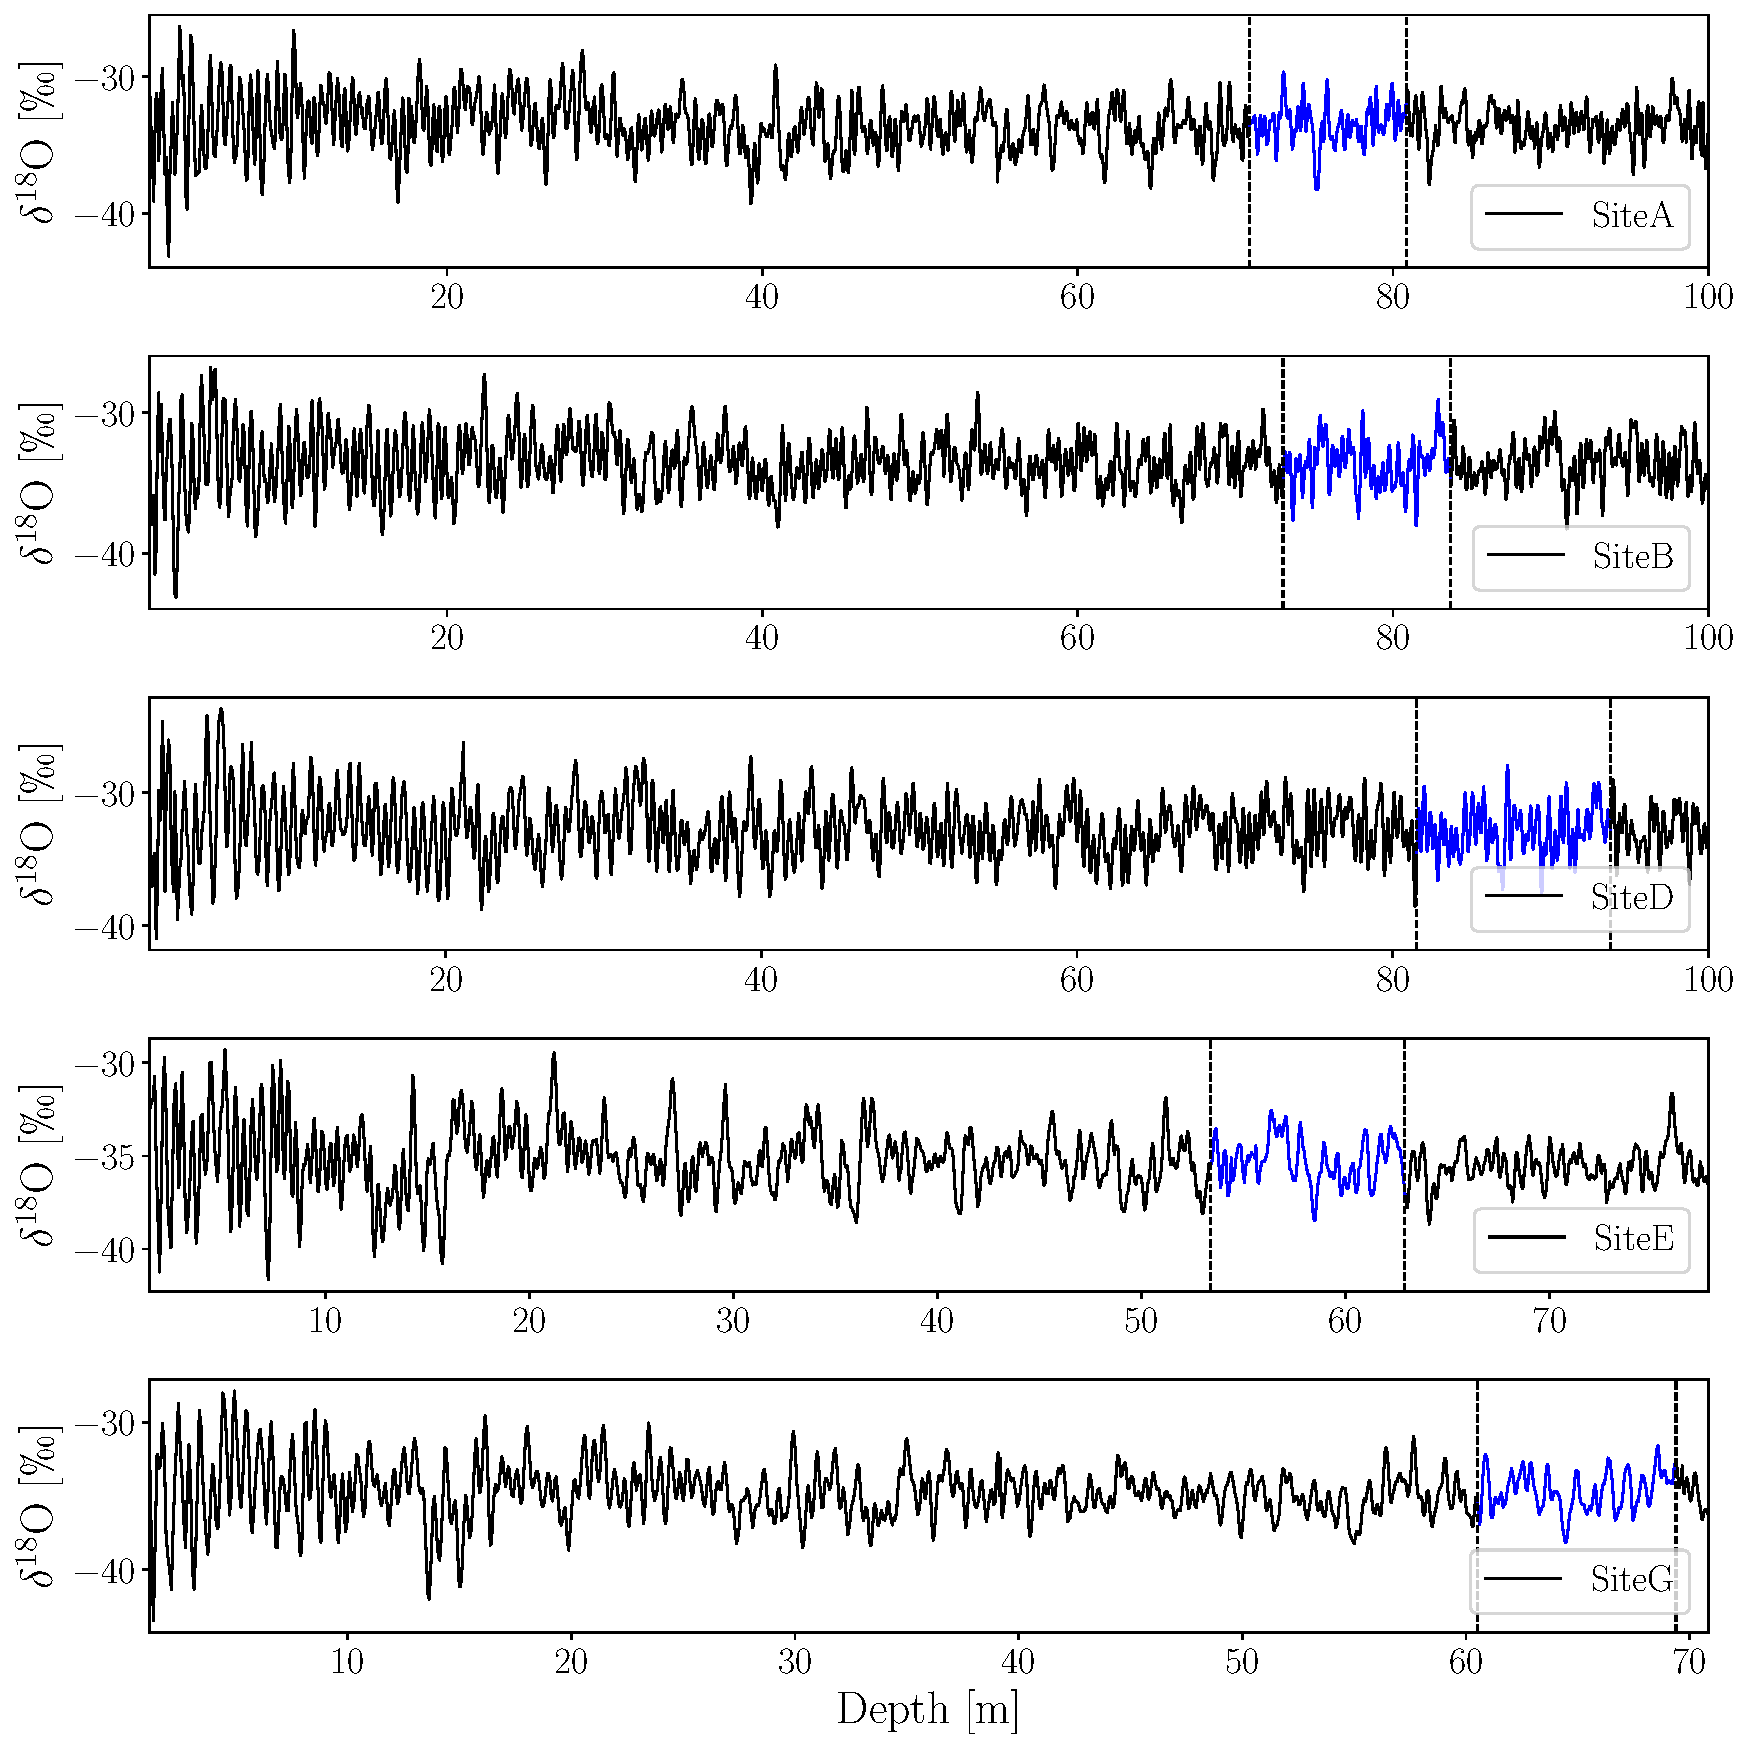
\includegraphics[width=0.8\textwidth]{AllAlphabetCores.pdf}
	\caption[All Alphabet core $\delta^{18}$O profiles in full.]{\small All Alphabet cores used in thesis in their full length. Blue sections correspond to depth of Laki to Tambora}
	\label{fig:AllAlphabetCores}
\end{figure}

The cores drilled in 1984-85 around the Crête core consist of the 400 m Crête core obtained in 1974 \cite{bibid} and eight shallow cores of varying length, between 25 m and 130 m, drilled in the Crête vicinity with a spatial coverage of 150 $\times$ 150 km, \cite[Clausen, Gundestrup, Johnsen 1988]{Clausen1988}. See Figures \ref{Fig:AlphabetCoresMap} and \ref{Fig:MapAlphabetCores} for spatial positioning of the ice cores.

Three cores were not of use for this project, Site C and Site F due to their shallow maximal depth, and the Crête core, as the ECM data were missing.
The remaining five cores make up cores in focus of this project. They are all well-documented, \cite[Clausen \& Hammer, 1988]{ClausenHammer1988}, \cite[Clausen, Gundestrup, Johnsen 1988]{Clausen1988}, and of high resolution making them ideal for the data and signal analysis used in the scope of this thesis. The Alphabet cores under consideration are presented in their full length in Figure \ref{fig:AllAlphabetCores}, and at the Laki to Tambora depth sections in Figure \ref{fig:AllAlphabetCores_LT}.


\begin{figure}[h]
	\centering
	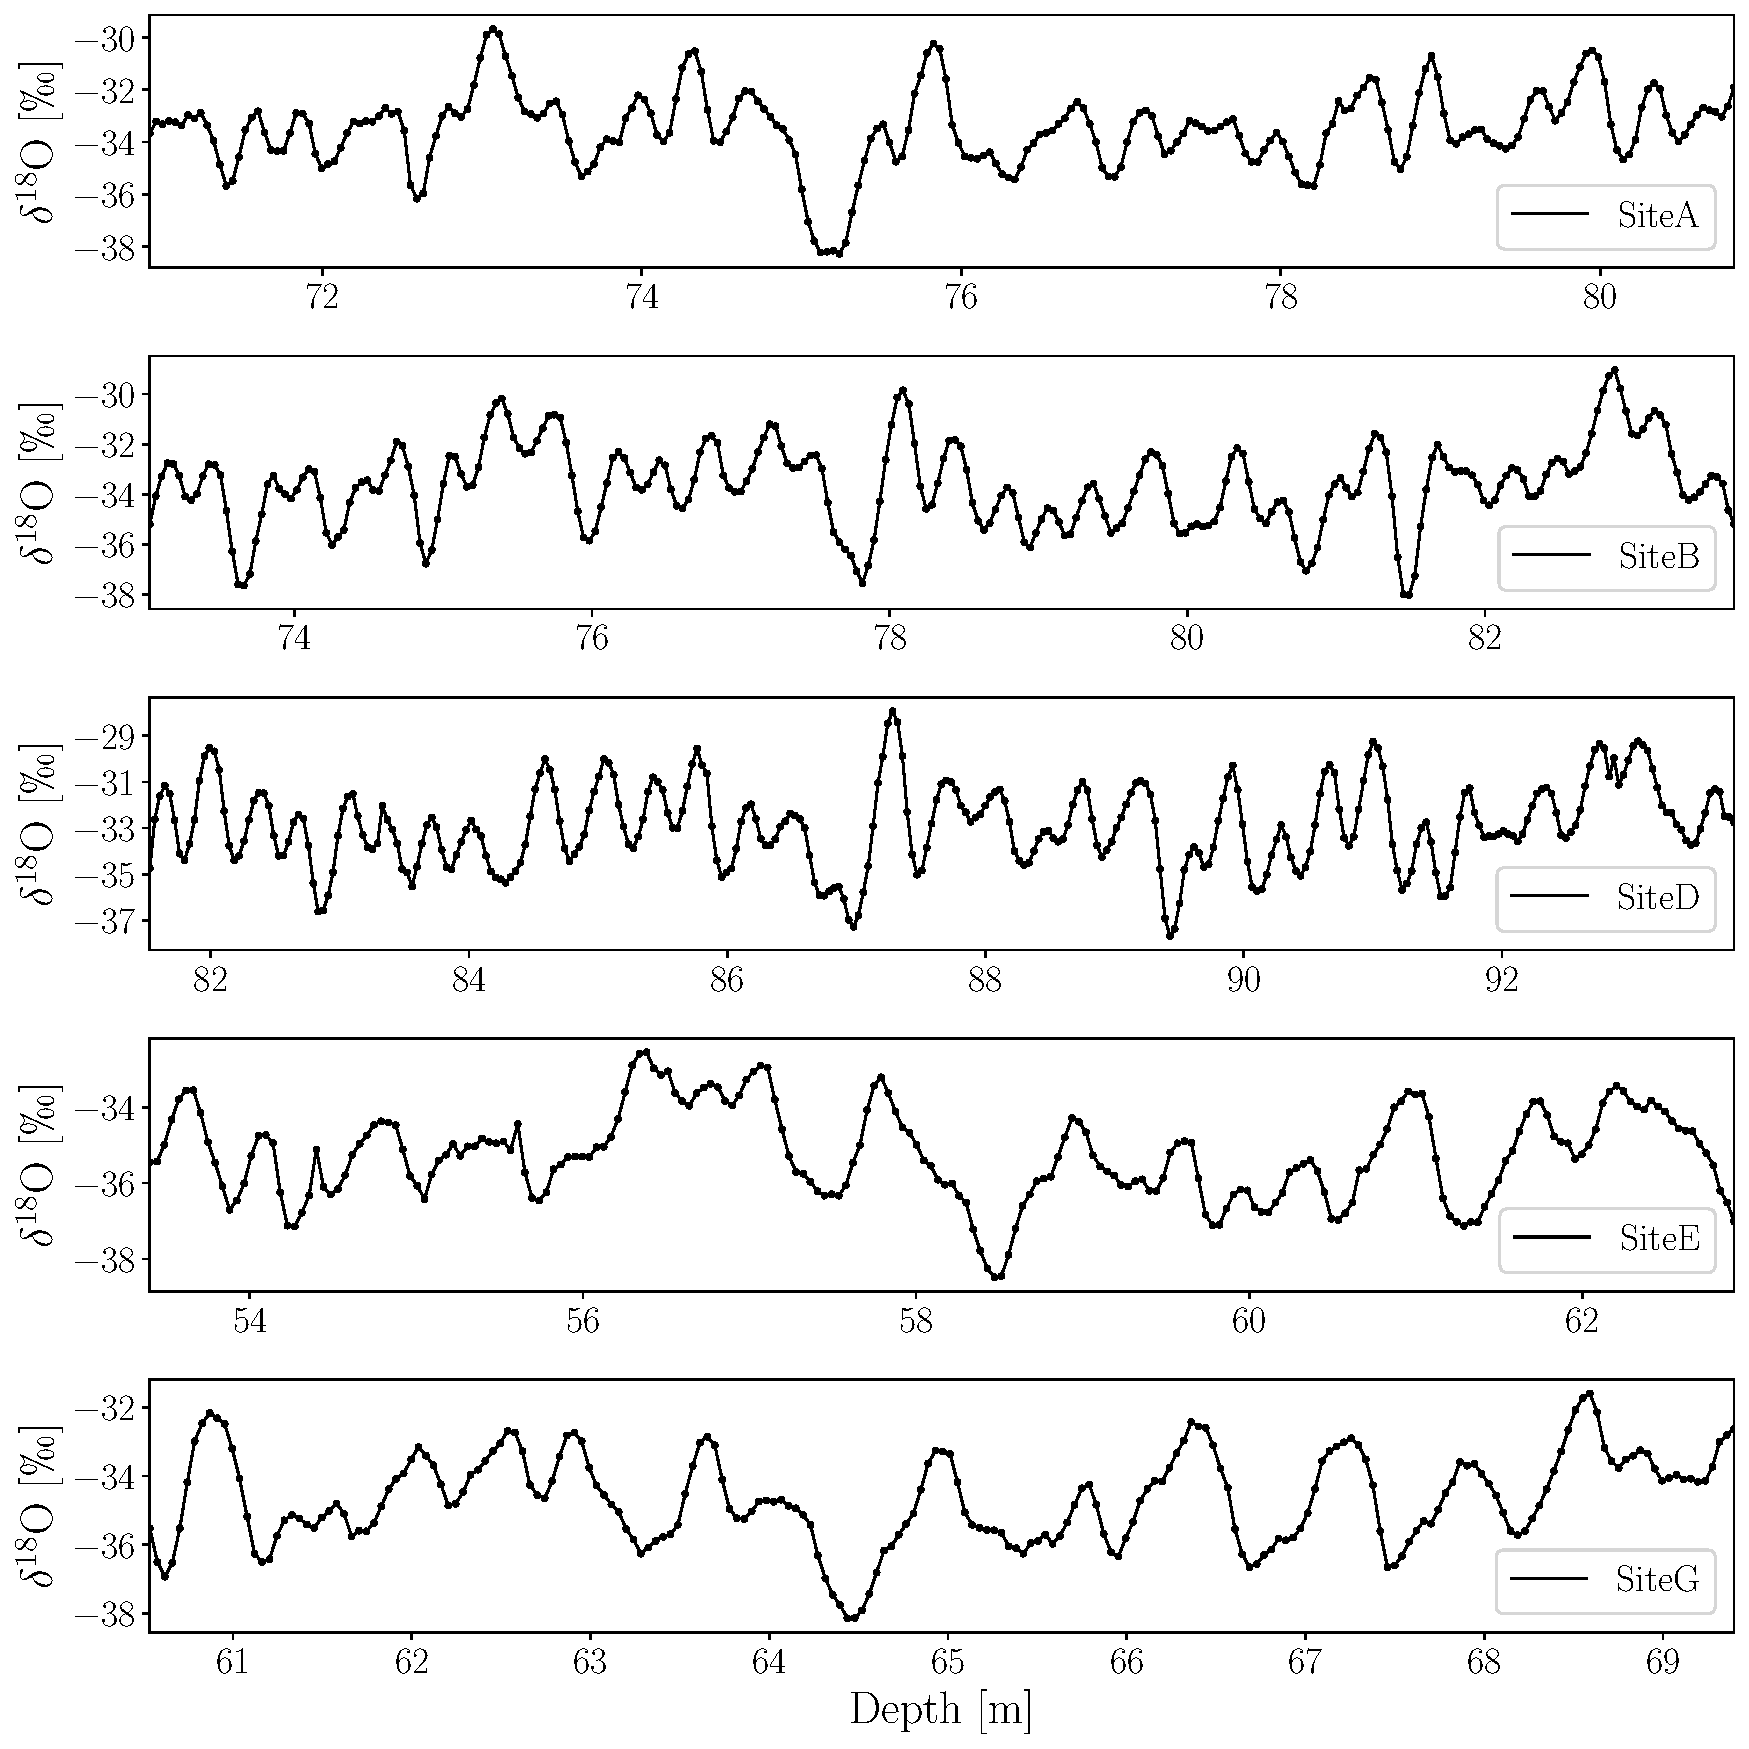
\includegraphics[width=0.8\textwidth]{AllAlphabetCores_LT.pdf}
	\caption[All Alphabet core $\delta^{18}$O profiles, depths from Laki to Tambora.]{\small All Alphabet cores used in thesis at the depth corresponding to Laki to Tambora.}
	\label{fig:AllAlphabetCores_LT}
\end{figure}



\subsubsection[Data Specifications][Data Specifications]{Data Specifications}
\label{Subsubsec:Data_Selection_Alhabet_Specifications}

The general specifications of all five cores, i.e. drill site information and volcanic event locations,are presented in table \ref{Tab:SiteA_CoreSpecs} [REFERENCE].
$d$ describes depth of event, $A$ describes accumulation rate, $T$ describes temperature, $\rho$ describes density at given depth and $s$ describes the width of a given event. Subscripts $L$ and $T$ stands for volcanic events Laki and Tambora, respectively, subscript $0$ describes initial surface condition, and superscripts $CH$ and $TQ$ represents the original and corrected values for depth and width of events.


%\begin{table}[h]
%	\centering
%	\begin{tabular}{l l|c}
%		\multicolumn{3}{c}{\textbf{Site A}} \\[0.1cm] 
%		\hline 
%		&& \\
%		$d_{L}^{CH}$ & [m] & 80.85 \\[0.15cm]
%		$d_{T}^{CH}$ & [m] & 70.9 \\[0.15cm]
%		$A_0$ W.E & [m] & 0.307 \\[0.15cm]
%		$A_0$ I.E. & [m] & 0.281519 \\[0.15cm]
%		$T_0$ & [$^{\text{o}}$C] & -29.41 \\[0.15cm]
%		$\rho_0$ & [$\text{kg}\,\text{m}^{-3}$] & 343.0\\[0.15cm]
%		$z_0$ & & 0.55 \\[0.15cm]
%		$s_L^{CH}$ & [cm] & 30.0 \\[0.15cm]
%		$s_T^{CH}$ & [cm] & 65.0 \\[0.15cm]
%		$\rho_L$ & [$\text{kg}\,\text{m}^{-3}$] & 836.0 \\[0.15cm]
%		$\rho_T$ & [$\text{kg}\,\text{m}^{-3}$] & 812.0 \\[0.15cm]		
%		$d_{L}^{TQ}$ & [m] & 80.87 \\[0.15cm]
%		$d_{T}^{TQ}$ & [m] & 70.90 \\[0.15cm]
%		$s_L^{TQ}$ & [cm] & 34.0 \\[0.15cm]
%		$s_T^{TQ}$ & [cm] & 40.0 \\[0.15cm]
%		
%	\end{tabular}
%	\caption[Core specifications, Site A.]{\small Core specifications for core drilled at Site A. $d$ describes depth of event, $A$ describes accumulation rate, $T$ describes temperature, $\rho$ describes density at given depth and $s$ describes the width of a given event. Subscripts $L$ and $T$ stands for volcanic events Laki and Tambora, respectively, subscript $0$ describes initial surface condition, and superscripts $CH$ and $TQ$ represents the original and corrected values for depth and width of events.}
%	\label{Tab:SiteA_CoreSpecs}
%\end{table}
	\begin{table}[h]
	\centering
	\begin{tabular}{l l|c c c c c}
		& & \textbf{Site A}& \textbf{Site B}& \textbf{Site D}& \textbf{Site E}& \textbf{Site G} \\[0.1cm]
		%\multicolumn{3}{c}{\textbf{Site A}} \\[0.1cm] 
		\hline 
		&&&&&& \\
		$d_{L}^{CH}$ & [m] & 80.85 & 83.7 & 93.8 & 62.95 & 69.4 \\[0.15cm]
		$d_{T}^{CH}$ & [m] & 70.9 & 73.0 & 81.5 & 53.4 & 60.5 \\[0.15cm]
		$A_0$ W.E & [m] & 0.307 & 0.327 & 0.365 & 0.225 & 0.251 \\[0.15cm]
		$A_0$ I.E. & [m] & 0.282 & 0.300 & 0.335 & 0.206 & 0.230 \\[0.15cm]
		$T_0$ & [$^{\text{o}}$C] & -29.41 & -29.77 & -28.3 & -30.37 & -30.1 \\[0.15cm]
		$\rho_0$ & [$\text{kg}\,\text{m}^{-3}$] & 343.0 & 355.0 & 350.0 & 325.0 & - \\[0.15cm]
		$z_0$ & & 0.55 & 0.55 & 0.825 & 0.675 & - \\[0.15cm]
		$s_L^{CH}$ & [cm] & 30.0 & 45.0 & 55.0 & 35.0 & 35.0 \\[0.15cm]
		$s_T^{CH}$ & [cm] & 65.0 & 55.0 & 70.0 & 40.0 & 75.0 \\[0.15cm]
		$\rho_L$ & [$\text{kg}\,\text{m}^{-3}$] & 836.0 & 841.0 & 857.0 & 786.0 & 807.0 \\[0.15cm]
		$\rho_T$ & [$\text{kg}\,\text{m}^{-3}$] & 812.0 & 816.0 & 839.0 & 749.0 & 778.0 \\[0.15cm]		
		$d_{L}^{TQ}$ & [m] & 80.87 & 83.82 & 93.95 & 62.9 & 69.38 \\[0.15cm]
		$d_{T}^{TQ}$ & [m] & 70.90 & 73.01 & 81.55 & 53.43 & 60.48\\[0.15cm]
		$s_L^{TQ}$ & [cm] & 34.0 & 30.0 & 30.0 & 45.0 & 35.0 \\[0.15cm]
		$s_T^{TQ}$ & [cm] & 40.0 & 57.0 & 55.0 & 48.0 & 82.0 \\[0.15cm]
		
	\end{tabular}
	\caption[Core specifications for core drilled at Site A.]{\small Core specifications for core drilled at Site A. $d$ describes depth of event, $A$ describes accumulation rate, $T$ describes temperature, $\rho$ describes density at given depth and $s$ describes the width of a given event. Subscripts $L$ and $T$ stands for volcanic events Laki and Tambora, respectively, subscript $0$ describes initial surface condition, and superscripts $CH$ and $TQ$ represents the original and corrected values for depth and width of events.}
	\label{tab:InterpSamples}
\end{table}
%\marginnote{%
%	\footnotesize
%	\centering
%	\begin{tabular}{l l|c}
%		\multicolumn{3}{c}{\textbf{Site A}} \\[0.1cm] 
%		\hline 
%		&& \\
%		$d_{L}^{CH}$ & [m] & 80.85 \\[0.13cm]
%		$d_{T}^{CH}$ & [m] & 70.9 \\[0.13cm]
%		$A_0^{\text{WE}}$ & [m] & 0.307 \\[0.13cm]
%		$A_0^{\text{IE}}$ & [m] & 0.282 \\[0.13cm]
%		$T_0$ & [$^{\text{o}}$C] & -29.41 \\[0.13cm]
%		$\rho_0$ & [$\text{kg}/\text{m}^{3}$] & 343.0\\[0.13cm]
%		$z_0$ & & 0.55 \\[0.13cm]
%		$s_L^{CH}$ & [cm] & 30.0 \\[0.13cm]
%		$s_T^{CH}$ & [cm] & 65.0 \\[0.13cm]
%		$\rho_L$ & [$\text{kg}/\text{m}^{3}$] & 836.0 \\[0.13cm]
%		$\rho_T$ & [$\text{kg}/\text{m}^{3}$] & 812.0 \\[0.13cm]		
%		$d_{L}^{TQ}$ & [m] & 80.87 \\[0.13cm]
%		$d_{T}^{TQ}$ & [m] & 70.90 \\[0.13cm]
%		$s_L^{TQ}$ & [cm] & 34.0 \\[0.13cm]
%		$s_T^{TQ}$ & [cm] & 40.0 \\[0.13cm]
%		
%	\end{tabular}
%	\captionof{table}[Core specifications, Site A.]{\footnotesize Core specifications for core drilled at Site A. $d$ describes depth of event, $A$ describes accumulation rate, $T$ describes temperature, $\rho$ describes density at given depth and $s$ describes the width of a given event. Subscripts $L$ and $T$ stands for volcanic events Laki and Tambora, respectively, subscript $0$ describes initial surface condition, and superscripts $CH$ and $TQ$ represents the original and corrected values for depth and width of events.}
%	\label{tab:InterpSamples}
%}[0.5cm]%





\end{document}